
\documentclass[a4paper,11pt]{article}
\usepackage[a4paper, margin=8em]{geometry}

% usa i pacchetti per la scrittura in italiano
\usepackage[french,italian]{babel}
\usepackage[T1]{fontenc}
\usepackage[utf8]{inputenc}
\frenchspacing 

% usa i pacchetti per la formattazione matematica
\usepackage{amsmath, amssymb, amsthm, amsfonts}

% usa altri pacchetti
\usepackage{gensymb}
\usepackage{hyperref}
\usepackage{standalone}

% imposta il titolo
\title{Appunti Fondamenti di Automatica}
\author{Luca Seggiani}
\date{2025}

% disegni
\usepackage{pgfplots}
\pgfplotsset{width=10cm,compat=1.9}

% imposta lo stile
% usa helvetica
\usepackage[scaled]{helvet}
% usa palatino
\usepackage{palatino}
% usa un font monospazio guardabile
\usepackage{lmodern}

% tikz in sans
\tikzset{every picture/.style={/utils/exec={\sffamily}}}

\renewcommand{\rmdefault}{ppl}
\renewcommand{\sfdefault}{phv}
\renewcommand{\ttdefault}{lmtt}

% circuiti
\usepackage{circuitikz}
\usetikzlibrary{babel}

% disponi il titolo
\makeatletter
\renewcommand{\maketitle} {
	\begin{center} 
		\begin{minipage}[t]{.8\textwidth}
			\textsf{\huge\bfseries \@title} 
		\end{minipage}%
		\begin{minipage}[t]{.2\textwidth}
			\raggedleft \vspace{-1.65em}
			\textsf{\small \@author} \vfill
			\textsf{\small \@date}
		\end{minipage}
		\par
	\end{center}

	\thispagestyle{empty}
	\pagestyle{fancy}
}
\makeatother

% disponi teoremi
\usepackage{tcolorbox}
\newtcolorbox[auto counter, number within=section]{theorem}[2][]{%
	colback=blue!10, 
	colframe=blue!40!black, 
	sharp corners=northwest,
	fonttitle=\sffamily\bfseries, 
	title=Teorema~\thetcbcounter: #2, 
	#1
}

% disponi definizioni
\newtcolorbox[auto counter, number within=section]{definition}[2][]{%
	colback=red!10,
	colframe=red!40!black,
	sharp corners=northwest,
	fonttitle=\sffamily\bfseries,
	title=Definizione~\thetcbcounter: #2,
	#1
}

% disponi problemi
\newtcolorbox[auto counter, number within=section]{problem}[2][]{%
	colback=green!10,
	colframe=green!40!black,
	sharp corners=northwest,
	fonttitle=\sffamily\bfseries,
	title=Problema~\thetcbcounter: #2,
	#1
}

% disponi codice
\usepackage{listings}
\usepackage[table]{xcolor}

\lstdefinestyle{codestyle}{
	backgroundcolor=\color{black!5}, 
	commentstyle=\color{codegreen},
	keywordstyle=\bfseries\color{magenta},
	numberstyle=\sffamily\tiny\color{black!60},
	stringstyle=\color{green!50!black},
	basicstyle=\ttfamily\footnotesize,
	breakatwhitespace=false,         
	breaklines=true,                 
	captionpos=b,                    
	keepspaces=true,                 
	numbers=left,                    
	numbersep=5pt,                  
	showspaces=false,                
	showstringspaces=false,
	showtabs=false,                  
	tabsize=2
}

\lstdefinestyle{shellstyle}{
	backgroundcolor=\color{black!5}, 
	basicstyle=\ttfamily\footnotesize\color{black}, 
	commentstyle=\color{black}, 
	keywordstyle=\color{black},
	numberstyle=\color{black!5},
	stringstyle=\color{black}, 
	showspaces=false,
	showstringspaces=false, 
	showtabs=false, 
	tabsize=2, 
	numbers=none, 
	breaklines=true
}

\lstdefinelanguage{javascript}{
	keywords={typeof, new, true, false, catch, function, return, null, catch, switch, var, if, in, while, do, else, case, break},
	keywordstyle=\color{blue}\bfseries,
	ndkeywords={class, export, boolean, throw, implements, import, this},
	ndkeywordstyle=\color{darkgray}\bfseries,
	identifierstyle=\color{black},
	sensitive=false,
	comment=[l]{//},
	morecomment=[s]{/*}{*/},
	commentstyle=\color{purple}\ttfamily,
	stringstyle=\color{red}\ttfamily,
	morestring=[b]',
	morestring=[b]"
}

% disponi sezioni
\usepackage{titlesec}

\titleformat{\section}
{\sffamily\Large\bfseries} 
{\thesection}{1em}{} 
\titleformat{\subsection}
{\sffamily\large\bfseries}   
{\thesubsection}{1em}{} 
\titleformat{\subsubsection}
{\sffamily\normalsize\bfseries} 
{\thesubsubsection}{1em}{}

% disponi alberi
\usepackage{forest}

\forestset{
	rectstyle/.style={
		for tree={rectangle,draw,font=\large\sffamily}
	},
	roundstyle/.style={
		for tree={circle,draw,font=\large}
	}
}

% disponi algoritmi
\usepackage{algorithm}
\usepackage{algorithmic}
\makeatletter
\renewcommand{\ALG@name}{Algoritmo}
\makeatother

% disponi numeri di pagina
\usepackage{fancyhdr}
\fancyhf{} 
\fancyfoot[L]{\sffamily{\thepage}}

\makeatletter
\fancyhead[L]{\raisebox{1ex}[0pt][0pt]{\sffamily{\@title \ \@date}}} 
\fancyhead[R]{\raisebox{1ex}[0pt][0pt]{\sffamily{\@author}}}
\makeatother

\begin{document}

% sezione (data)
\section{Lezione del 26-03-25}

% stili pagina
\thispagestyle{empty}
\pagestyle{fancy}

% testo
\subsection{Trasformata di Laplace ed equazioni differenziali}
Vediamo come applicare la trasformata di Laplace nella risoluzione delle equazioni differenziali ordinarie.

\subsubsection{Esempio: risposta al gradino di un sistema del primo ordine}
Prendiamo quindi un equazione differenziale del primo ordine e vediamone la trasformazione nel domino di Laplace:
$$
a_1 \frac{dy}{dt} + a_0 f(t) = b_0 u, \quad y(0) = 0
$$
Ricordiamo quindi la trasformata di Laplace della derivata:
$$
\mathcal{L}\left\{ \frac{dy}{dt} \right\} = sY(s) - y(0) = sY(s)
$$
nel nostro caso $y(0) = 0$.
Otteniamo allora:
$$
a_1 \cdot s Y(s) + a_0 \cdot Y(s) = b_0 \cdot U(s)
$$

Notiamo che quest'equazione non è più differenziale, e possiamo quindi risolverla per via algebrica.Troviamo allora la funzione di trasferimento $G(s)$ come il rapporto uscita/ingresso:
$$
\frac{Y(s)}{U(s)} = \frac{b_0}{a_0 + a_1 s} = G(s) 
$$
L'uscita sarà allora data da:
$$
Y(s) = G(s) \cdot U(s)
$$

Otteniamo ad esempio la risposta a $u(t) = H(t)$, cioè al gradino di trasformata $U(s) = \frac{1}{s}$:
$$
Y(s) = G(s) \cdot \frac{1}{s} = \frac{b_0}{s (a_0 + a_1 s)}
$$

Possiamo applicare il teorema del valor iniziale e del valor finale per verificare, rispettivamente, l'aderenza alle condizioni iniziali ($y(0) = 0$) e l'andamento a $t \rightarrow +\infty$:
\begin{itemize}
	\item Valor iniziale:
		$$
		\lim_{s \rightarrow + \infty} s \cdot Y(s) = 0 =\lim_{t \rightarrow 0} y(t)
		$$
	\item Valor finale:
		$$
		\lim_{s \rightarrow 0} s \cdot Y(s) = \frac{b_0}{a_0} =\lim_{t \rightarrow +\infty} y(t)
		$$
\end{itemize}

Calcoliamo quindi l'antitrasformata.
Rendiamo innanzitutto il polinomio al denominatore \textit{monico}, e scomponiamo:
$$
= \frac{\frac{b_0}{a_1}}{s \left( \frac{a_0}{a_1} + s \right)} = \frac{A}{s} + \frac{B}{\frac{a_0}{a_1} + s}
$$
con:
$$
A = \lim_{s \rightarrow 0} s \cdot \frac{b_0}{s(a_0 + a_1 s)} = \frac{b_0}{a_0}
$$
$$
B = \lim_{s \rightarrow -\frac{a_0}{a_1}} \left( s + \frac{a_0}{a_1} \right)  \frac{\frac{b_0}{a_1}}{s \left( \frac{a_0}{a_1} + s \right)} = -\frac{b_0}{a_0}
$$
da cui:
$$
Y(s) = \frac{b_0}{a_0 s} - \frac{b_0}{a_0 \left( s + \frac{a_0}{a_1} \right)}
$$
e l'antitrasformata:
$$
\mathcal{L}^{-1} \left\{ Y(s) \right\} = \frac{b_0}{a_0} \left( 1 - e^{-\frac{a_0}{a_1}t} \right) \cdot H(t)
$$
Notiamo che questo rispetta le condizioni iniziali, e quindi il teorema del valor iniziale, nonché il limite ad infinito posto dal teorema del valor finale.

\subsubsection{Parametri significativi dei sistemi del primo ordine}
Possiamo dare ad alcune delle grandezze trovate dei nomi significativi dal punto di vista delle grandezze.
Ad esempio, introdurremo:
\begin{itemize}
	\item Il \textbf{guadagno statico} $G(0) = \frac{b_0}{a_0}$;
	\item La \textbf{costante tempo}, o \textit{tempo caratteristico} $T$, data da $\frac{1}{T} = \frac{a_0}{a_1}$.
\end{itemize}

Questo ci permette di riscrivere la risposta $y(t)$ come:
$$
y(t) = G(0) \left( 1 - e^{-\frac{t}{T}} \right)
$$

In particolare, avremo che il valore di $y(T)$ al tempo caratteristico $T$ sarà approssimativamente il $63.2 \%$ del valore del guadagno statico $G(0)$.

Potremmo chiederci il perché di una costante apparentemente così arbitraria.
Ipotizzando che al tempo $T$ si raggiunga una qualche frazione del guadagno $G(0)$, allora, impostiamo:
$$
y(T) = k \cdot G(0) \implies k = \frac{y(T)}{G(0)} = \frac{\frac{b_0}{a_0} \left( 1 - e^{-\frac{a_0}{a_1} \cdot \frac{a_1}{a_0}} \right) }{\frac{b_0}{a_0}} = 1 - e^{-1} \approx 0.632
$$
che è esattamente la costante di prima.
Possiamo generalizzare questo procedimento a multipli arbitrari di $T$, $\mu T$:
$$
y(\mu T) = k \cdot G(0) \implies k = \frac{y(\mu T)}{G(0)} = \frac{\frac{b_0}{a_0} \left( 1 - e^{-\frac{a_0}{a_1} \cdot \mu \frac{a_1}{a_0}} \right) }{\frac{b_0}{a_0}} = 1 - e^{-\mu} 
$$
ricavando quindi una funzione:
$$
p(\mu) = 1 - e^{-\mu}
$$
per la percentuale $p(\mu)$ di guadagno raggiunta al multiplo $\mu$-esimo del tempo caratteristico $T$. 
Questa valore ottiene i seguenti valori per un insieme di $\mu$ selezionato:
\begin{table}[H]
	\center \rowcolors{2}{white}{black!10}
	\begin{tabular} { c | c }
		$\mu$ & $p(\mu)$ \\
		\hline 
		0 & 0 \\ 
		1 & $63.2 \% $ \\
		2 & $86.5 \% $ \\
		3 & $95 \% $ \\
		4 & $98.2 \% $ \\
	\end{tabular}
\end{table}
che chiaramente tende, ma non raggiunge mai, il $100 \%$ nel limite a infinito.

\noindent
\begin{minipage}{\textwidth}
	Possiamo quindi tracciare un grafico dell'andamento di $y(t)$ in Python, evidenziando il valore raggiunto in $t = T$:
	\begin{center}
		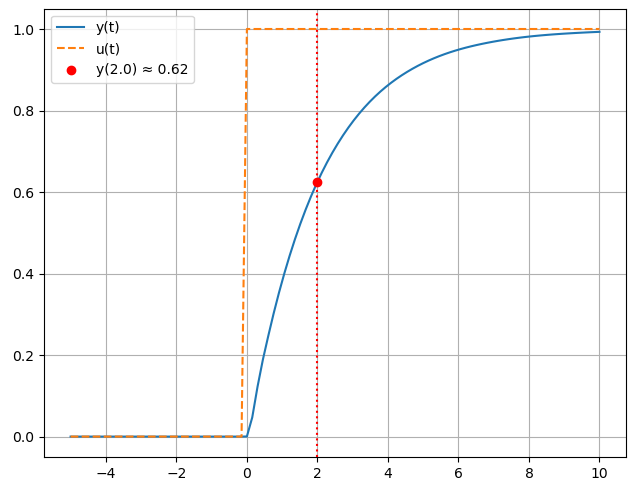
\includegraphics[scale=0.62]{../figures/first_degree_step_response.png}
	\end{center}
	che risulta effettivamente abbastanza vicino al $\sim 63.2 \%$.
\end{minipage}

\subsubsection{Tempo di assestamento}
Un'altro valore di interesse è il \textbf{tempo di assestamento} alla percentuale $i$, inteso come il tempo che serve a un sistema dinamico per rimanere una fascia $\pm i \%$ attorno al valore di regime.

Ad esempio, se vogliamo calcolare il tempo di assestamento al $5\%$, possiamo dire:
$$
y(t) = G(0) \left( 1 - e^{-\frac{t_{ss}}{T}} \right) = 0.95 \cdot G(0) \implies 0.05 = e^{-\frac{t_{ss}}{T}}
$$
da cui:
$$
t_{ss} = T \cdot \ln(20) \approx 3T
$$
cioè 3 volte il tempo caratterstico, come risultava abbastanza chiaro dalla tabella del paragrafo precedente.

\subsection{Forme di Bode e di Evans}
Vediamo un'altra equazione differenziale, dove adesso compare la derivata dell'ingresso:
$$
a_1 \frac{dy}{dt} + a_0 y = b_1 \frac{du}{dt} + b_0 u
$$
Nel dominio di Laplace questa avrà l'aspetto:
$$
a_1 \cdot s Y(s) + a_0 \cdot Y(s) + b_1 \cdot s U(s) + b_0 \cdot U(s)
$$
da cui la funzione di trasferimento:
$$
\frac{Y(s)}{U(s)} = \frac{b_0 + b_1 s}{a_0 + a_1 s} = G(s)
$$

Nota questa funzione di trasferimento, possiamo riportare due forme standard di riscrittura, che ne evidenziano proprietà diverse:
\begin{itemize}
	\item \textbf{Forma di Bode:} evidenzia le costanti tempo del sistema dinamico.
		$$
		G(s) = \frac{b_0}{a_0} \frac{1 + s \cdot \frac{b_1}{b_0}}{1 + s \cdot \frac{a_1}{a_0}} = G(0) \cdot \frac{1 + s \cdot \tau_z}{1 + s \cdot \tau}
		$$
		Notiamo che l'effetto della derivata dell'ingresso è stato quello di portare un termine $s$ al numeratore, e quindi quello di introdurre uno zero (a $-\frac{b_0}{b_1}$) nella funzione di trasferimento (zero per cui abbiamo introdotto il tempo caratteristico $\tau_z$).
	\item \textbf{Forma di Evans:} evidenzia le singolarità dinamiche del sistema, ovvero poli e zeri:
		$$
		G(s) = \frac{b_1}{a_1} \cdot \frac{s + \frac{b_0}{b_1}}{s + \frac{a_0}{a_1}}
		$$
\end{itemize}

Ad esempio, riguardo alla funzione di trasferimento dell'esempio 12.1.1, che ricordiamo essere:
$$
G(s) = \frac{\frac{b_0}{a_0}}{s + \frac{a_0}{a_1}}
$$
possiamo dire che si trova già in \textit{forma di Evans}, in quanto al denominatore è esplicitato l'unico polo.

Per ricavare la forma di Bode, invece, vorremo esporre il termine tempo caratteristico $\tau = \frac{a_1}{a_0}$:
$$
G(s) = \frac{b_0}{a_0} \cdot \frac{1}{1 + s \cdot \frac{a_1}{a_0}}
$$
che è nuovamente:
$$
= G(0) \cdot \frac{1}{1 + s \cdot \tau}
$$

\subsection{Sistemi del secondo ordine}
Abbiamo visto finora sistemi del primo ordine risolti tramite la trasformata di Laplace.
Vediamo adesso il caso dei sistemi del secondo ordine, che ci permettono di modellizzare una vasta gamma di fenomeni di interesse ingegneristico:
$$
a_2 \frac{d^2 y}{dt^2} + a_1 \frac{dy}{dt} + a_0 y = b_0 u
$$
complicando la situazione con condizioni iniziali non nulle ($y(0), y'(0) \neq 0$).

Applichiamo quindi Laplace alle due derivate successive:
$$
\mathcal{L} \left\{ \frac{dy}{dt} \right\} = s \cdot Y(s) - y(0)
$$
$$
\mathcal{L} \left\{ \frac{d^2y}{dt^2} \right\} = s \left( Y(s) - y(0) \right) - y'(0)
$$
da cui ricaviamo la forma:
$$
a_2 \cdot \left( s^2 \cdot Y(s) - s \cdot y(0) - y'(0) \right) + a_1 \cdot \left( s \cdot Y(s) - y(0) \right) + a_0 \cdot Y(s) = b_0 \cdot U(s)
$$

Esplicitando $Y(s)$ si otterrà:
$$
Y(s) = \frac{a_2 s \cdot y(0) + a_2 \cdot y'(0) + a_1 \cdot y(0)}{a_0 + a_1 s + a_2 s^2} + \frac{b_0}{a_0 + a_1 s + a_2 s^2} U(s) 
$$
dove riconosciamo che il primo termine rappresenta la \textbf{risposta libera} e il secondo la \textbf{risposta forzata} del sistema. 

Decidiamo di concentrarci sulla risposta forzata, ricavando la funzione di trasferimento:
$$
G(s) = \frac{Y(s)}{U(s)} = \frac{b_0}{a_2 s^2 + a_1 s + a_0} = \frac{ \frac{b_0}{a_2} }{s^2 + \frac{a_1}{a_2}s + \frac{a_0}{a_2}}
$$
da cui i poli al denominatore:
$$
p_{1, 2} = - \frac{-a_1 \pm \sqrt{a_1^2 - 4 a_0 a_2}}{2 a_2}
$$
da cui notiamo che 1) non ci interessa di considerare per i polinomi il polinomio monico, in quanto la loro posizione non cambierà e 2) prendiamo il segno $-$, in quanto vogliamo scrivere:
$$
G(s) = \frac{ \frac{b_0}{a_2} }{(s + p_1) (s + p_2)}
$$

Potremo quindi individuare il \textbf{determinante}:
$$
\Delta = a_1^2 - 4a_0a_2
$$
sulla base del quale distinguiamo 3 situazioni:
\begin{itemize}
	\item $\Delta > 0$, si hanno 2 poli \textbf{reali distinti}.
	\item $\Delta = 0$, si hanno 2 poli \textbf{reali coincidenti};
	\item $\Delta < 0$, si hanno 2 poli \textbf{complessi coniugati};
\end{itemize}
Vediamo nel dettaglio queste situazioni.

\subsubsection{$\mathbf{\Delta > 0}$, 2 poli reali distinti}
Risulta immediato che:
$$G(0) = \frac{b_0}{a_0}$$
e definiamo poi:
$$
\quad T_1 = \frac{1}{p_1}, \quad T_2 = \frac{1}{p_2}
$$

Vogliamo innanzitutto vedere come portarci nelle forme di Bode e di Evans.
Prima di tutto, però, dimostriamo due importanti proprietà:
\begin{enumerate}
	\item $p_1 \cdot p_2 = \frac{1}{T_1 \cdot T_2} = \frac{a_0}{a_2}$ \par\smallskip 
		Il lato sinistro è chiaro dalla definizione di $T_1$ e $T_2$.
		Per dimostrare il lato destro calcoliamo direttamente $p_1 \cdot p_2$:
		$$
		p_1 \cdot p_2 = \left( - \frac{-a_1 + \sqrt{a_1^2 - 4 a_0 a_2}}{2 a_2} \right) \left( - \frac{-a_1 - \sqrt{a_1^2 - 4 a_0 a_2}}{2 a_2} \right)
		$$
		$$
		= \frac{1}{4a_2^2} \left( a_1^2 - a_1^2 + 4a_2a_0 \right) = \frac{a_2 a_0}{a_2^2} = \frac{a_0}{a_2}
		$$ \qed
		
	\item $p_1 + p_2 = \frac{1}{T_1} + \frac{1}{T_2} = \frac{a_1}{a_2}$ \par\smallskip
		Anche qui il lato sinistro è chiaro dalla definizione di $T_1$ e $T_2$.
		Per dimostrare il lato destro procediamo nuovamente per calcolo diretto:
		$$
		p_1 + p_2 = - \frac{-a_1 + \sqrt{a_1^2 - 4 a_0 a_2}}{2 a_2} + \left( - \frac{-a_1 - \sqrt{a_1^2 - 4 a_0 a_2}}{2 a_2} \right) = \frac{a_1}{2 a_2} + \frac{a_1}{2 a_2} = \frac{a_1}{a_2}
		$$ \qed
\end{enumerate}

Vediamo allora le forme standard:
\begin{itemize}
	\item \textbf{Forma di Bode:} è analoga a quella vista nel caso lineare, cioè:
	$$
	G(s) = G(0) \cdot \frac{1}{(1 + s \cdot T_1)(1 + s \cdot T_2)}
	$$
	la validità di questa si ricava a moltiplicando e dividendo per $T_1 T_2$ e applicando la proprietà 1:
	$$
	= \frac{b_0}{a_0} \cdot \frac{1}{T_1 T_2 (\frac{1}{T_1} + s)(\frac{1}{T_2} + s)} = \frac{b_0}{a_0} = \frac{b_0}{a_0} \cdot \frac{a_0}{a_2} \cdot \frac{1}{(s + p_1)(s + p_2)} = \frac{\frac{b_0}{a_2}}{(s + p_1)(s + p_2)}
	$$ 
	che riconosciamo essere la forma che abbiamo usato finora.
	\qed
	\item \textbf{Forma di Evans:} è la forma a poli espliciti che avevamo già trovato:
	$$
	G(s) = \frac{\frac{b_0}{a_2}}{(s + p_1)(s + p_2)}
	$$
\end{itemize}

\par\medskip

Vediamo quindi la \textbf{risposta al gradino}:
$$
Y(s) = G(s) \cdot U(s) = \frac{\frac{b_0}{a_2}}{(s + \frac{1}{T_1})(s + \frac{1}{T_2}) \cdot s} = \frac{A}{s} + \frac{B}{s + \frac{1}{T_1}} + \frac{C}{s + \frac{1}{T_2}}
$$
dove si è adottata questa forma \textit{"ibrida"} di Evans, dove manteniamo esplicite le costanti tempo.

Calcoliamo quindi i residui:
$$
A = \lim_{s \rightarrow 0} \frac{\frac{b_0}{a_2}}{(s + \frac{1}{T_1})(s + \frac{1}{T_2})} = \frac{b_0}{a_2} \cdot T_1 \cdot T_2 = \frac{b_0 \cdot a_2}{a_2 \cdot a_0} = \frac{b_0}{a_0} = G(0)
$$
sfruttando la proprietà 1 riportata prima.
Si ha poi:
$$
B = \lim_{s \rightarrow - \frac{1}{T_1}} \frac{\frac{b_0}{a_2}}{s (s + \frac{1}{T_2})} 
= \frac{b_0}{a_2} \cdot \frac{1}{-\frac{1}{T_1} (\frac{1}{T_2} - \frac{1}{T_1})} 
= \frac{b_0 \cdot T_1^2 T_2}{a_2 (T_2 - T_1)} 
= \frac{T_1}{T_2 - T_1} \cdot G(0)
$$
$$
C = \lim_{s \rightarrow - \frac{1}{T_2}} \frac{\frac{b_0}{a_2}}{s (s + \frac{1}{T_1})} 
= \frac{b_0}{a_2} \cdot \frac{1}{-\frac{1}{T_2} (\frac{1}{T_1} - \frac{1}{T_2})} 
= \frac{b_0 \cdot T_1 T_2^2}{a_2 (T_2 - T_1)} 
= -\frac{T_2}{T_2 - T_1} \cdot G(0)
$$

Calcoliamo quindi l'antitrasformata:
$$
y(t) = \mathcal{L}^{-1} \{ G(s) \cdot U(s) \} = G(0) \cdot \left( 1 + \frac{T_1 e^{-\frac{t}{T_1}} - T_2 e^{-\frac{t}{T_2}}}{T_2 - T_1} \right) \cdot H(t)
$$

# magari un grafichino

Notiamo che il grafico è qualitativamente simile a quello ottenuto da un sistema del primo ordine, anche se dobbiamo distinguere non una ma due costanti di tempo, $T_1$ e $T_2$.

\end{document}
